\section{The $\Z_2$-Homology Cover}
\label{sec:homcover}

Now, let~$G$ be directed, and let $h$
be a homology signature.  In this section, we describe an
algorithm to compute a $\Z_2$-minimal \emph{cycle} with signature~$h$
in $(g+b)^{O(g+b)}n \log n$ time. Our algorithm can be
used as a subroutine to compute minimum-cost even subgraphs in
\emph{any} homology class in the same asymptotic running time
using a dynamic programming procedure described later in this section.
Again, by Lemma~\ref{lem:surface-st-cut}, our algorithm can be used to find a minimum $s,t$-cut in~$G^*$ in the same amount of time if~$G$ is undirected.

The algorithm of the previous section constructs and searches several relevant finite portions of the (infinite) universal cover of the input surface.
Instead of the universal cover, the algorithms of this section construct and search another canonical covering space, called the \emph{$\Z_2$-homology cover}.
We also use a generalization of Klein's seminal multiple-source shortest path algorithm~\cite{k-msspp-05} for planar graphs to higher-genus embedded graphs \cite{cce-msspe-13}.
\note{TODO(kylejfox): The top of page 2 in the SODA 2011 paper contains some good motivation for the homology cover technique. That material should be transferred either to here or the introduction. Also mention the shortest non-trivial directed cycle papers~\cite{e-sncds-11,f-sntcd-13} that use similar techniques.}

\subsection{The $\Z_2$-homology cover}
After computing homology signatures for each edge, the $\Z_2$-homology cover of a combinatorial surface can be defined using a standard~\emph{voltage construction}~\cite[Chapter 4]{gt-tgt-01}, as follows.  Let $\Gbar$ denote the graph whose vertices are all ordered pairs $(v, h)$ where $v$ is a vertex of $G$ and $h$ is an element of $(\Z_2)^\beta$, and whose edges are the ordered pairs $(\arc{u}{v}, h) := (u, h)\arcto(v, h\oplus [u\arcto v])$ for all edges $\arc{u}{v}$ of $G$ and all homology classes $h \in (\Z_2)^\beta$.  Let $\pi\colon \Gbar\to G$ denote the covering map $\pi(v, h) = v$; this map projects any cycle in $\Gbar$ to a cycle in $G$.  To define a cellular embedding of~$\Gbar$, we declare a cycle in $\Gbar$ to be a face if and only if its projection is a face of $G$.  The combinatorial surface defined by this embedding is the $\Z_2$-homology cover $\Sigmabar$.

Our construction can be interpreted more topologically as follows.  Let $\dualarc_1, \dots, \dualarc_\beta$ denote the system of dual arcs used to define the homology signatures $[e]$.  The surface $D := \Sigma\setminus(\dualarc_1\cup\cdots\cup \dualarc_\beta)$ is a topological disk.  Each arc $\dualarc_i$ appears on the boundary of $D$ as two segments $\dualarc^+_i$ and~$\dualarc^-_i$.  For each signature $h\in (\Z_2)^\beta$, we create a disjoint copy $(D,h)$ of $D$; for each index~$i$, let $(\dualarc^+_i, h)$ and $(\dualarc^-_i, h)$ denote the copies of $\dualarc^+_i$ and $\dualarc^-_i$ in the disk $(D, h)$.  For each index~$i$, let~$b_i$ denote the $\beta$-bit vector whose $i$th bit is equal $1$ and whose other $\beta-1$ bits are all equal to~$0$.  The $\Z_2$-homology cover $\Sigmabar$ is constructed by gluing the~$2^\beta$ copies of $D$ together by identifying boundary paths $(\dualarc^+_i,h)$ and $(\dualarc^-_i, h\oplus b_i)$, for every index $i$ and homology class $h$.  See Figure \ref{fig:cover-ex} for an example.

\begin{figure}
\centering
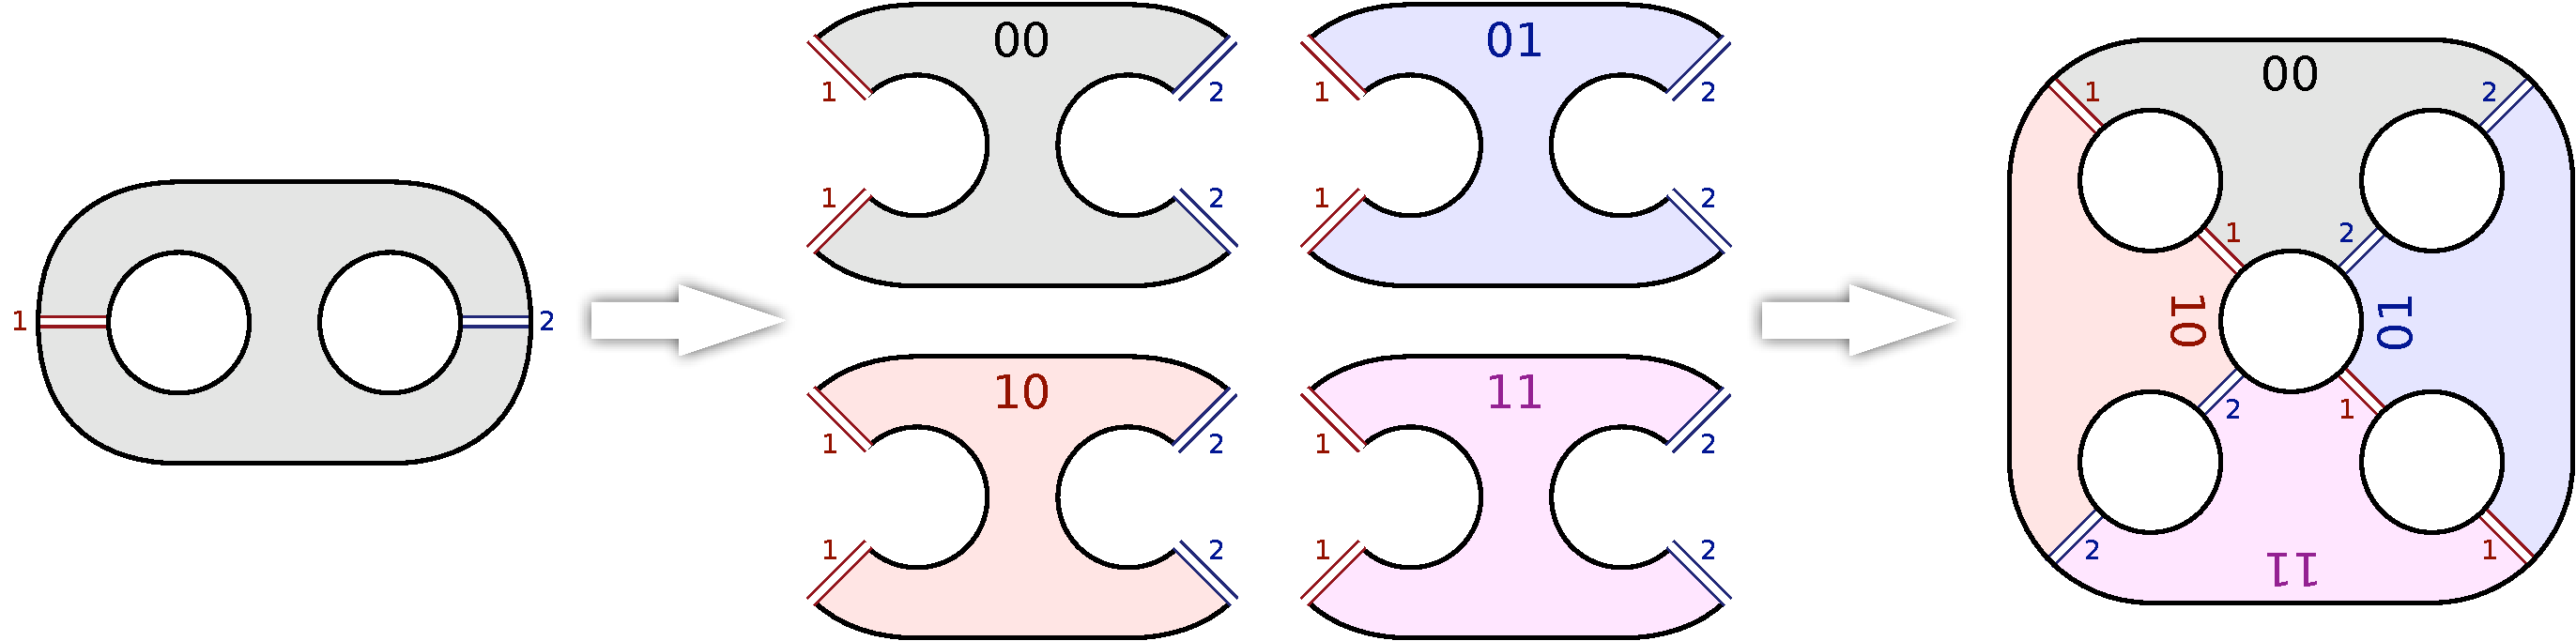
\includegraphics[height=1.5in]{Fig/hom-cover-example}
\caption{Constructing the $\Z_2$-homology cover of a pair of pants (a genus zero surface with three boundaries).}
\label{fig:cover-ex}
\end{figure}

\begin{lemma}
\label{lem:cover-cxy}
The combinatorial surface $\Sigmabar$ has $\nbar = 2^\beta n$ vertices, genus $\gbar = O(2^\beta \beta)$, and $\bbar = O(2^\beta b)$ boundaries, and it can be constructed in $O(2^\beta n)$ time.
\end{lemma}

\begin{proof}
Let $m$ and $f$ denote the number of edges and faces of $\Sigma$, respectively.  Recall that the Euler characteristic of $\Sigma$ is $\chi = n - m + f = 2 - 2g - b = 1-\beta$.  The combinatorial surface~$\Sigmabar$ has exactly $\nbar = 2^\beta n$ vertices, $2^\beta m$ edges, and $2^\beta f$ faces, so its Euler characteristic is $\chibar = 2^\beta (1-\beta)$.

If $b>1$, then each boundary cycle $\delta_i$ has a non-zero homology signature; at least one arc $\dualarc_j$ has exactly one endpoint on~$\delta_i$.  Thus, $\Sigmabar$ has exactly $\bbar = 2^{\beta-1} b$ boundary cycles, each of which is a double-cover (in fact, the $\Z_2$-homology cover) of some boundary cycle~$\delta_i$.  It follows that~$\Sigmabar$ has genus $\gbar = 1-(\chibar+\bbar)/2 = {2^{\beta-2} ({4g+b-4}) + 1}$.  (Somewhat surprisingly, $\Sigmabar$ may have positive genus even when $\Sigma$ does not!)  On the other hand, when $b=1$, the boundary cycle~$\delta_1$ is null-homologous, so $\Sigmabar$ has $\bbar = 2^\beta b$ boundary cycles, and thus~$\Sigmabar$ has genus $\gbar = {1-(\chibar+\bbar)/2} =  {2^\beta (g-1) + 1}$.

After computing the homology signatures for $\Sigma$ in $O(\beta n)$ time, following Lemma \ref{lem:sign}, it is straightforward to construct $\Sigmabar$ in $O(\nbar) = O(2^\beta n)$ time.
\end{proof}

We assign weights to the directed edges of $\Gbar$ by setting $\wbar(\arc{u}{v},h) := w(\arc{u}{v})$ for each edge $\arc{u}{v}$ of~$G$ and each homology class $h$.  In other words, each directed edge in $\Sigmabar$ inherits the weight of its projection in $\Sigma$.

Now consider an arbitrary path $\path$ in $G$, with (possibly equal) endpoints $u$~and $v$.  A straightforward induction argument implies that for any homology class $h \in (\Z_2)^\beta$, the path~$\path$ is the projection of a unique path from $(u,h)$ to $(v,h\oplus[\path])$, which we denote \EMPH{$(\path,h)$}.  Moreover, this lifted path has the same length as its projection: $w(\path) = \wbar(\path,h)$.  The following lemmas are now immediate.

\begin{lemma}
\label{lem:lift-shortest}
Every lift of a shortest directed path in $G$ is a shortest directed path in $\Gbar$.
\end{lemma}

\begin{lemma}
\label{lem:lift-minimal}
A loop $\ell$ in $G$ with basepoint $v$ is $\Z_2$-minimal if and only if, for every homology class $h\in (\Z_2)^\beta$, the lifted path $(\ell,h)$ is a shortest directed path in $\Gbar$ from $(v,h)$ to $(v,h\oplus[\ell])$.
\end{lemma}
